\chapter{Informationstheorie}
%TODO: Informationen zum Thema Informationstheorie aus ausführlichem Skript dgt_all einarbeiten
In der Informationstheorie geht es um die Definition und quantitative Bewertung von Information. Im Folgenden wird der Austausch von Informationen mittels Nachrichten über Kanäle besprochen. Ein Kommunikationssystem wird durch die Kommunikationspartner, der Kommunikationsrichtung und der Informationsart charakterisiert. Als Kommunikationsparter können Menschen und Maschinen auftreten. Die Kommunikationsrichtung wird allgemein mit simplex oder duplex beschrieben. Ist ein Kommunikationskanal simplex aufgebaut, so erfolgt das Senden der Nachrichten immer vom selben Kommunikationsteilnehmer. Als duplex werden Kommunikationskanäle bezeichnet über die beide Kommunikationspartner gleichzeitig einander Nachrichten senden und empfangen. Zusätzlich gibt es die Bezeichnung halb-duplex, damit ist gemeint, dass nicht gleichzeitig gesendet und empfangen werden kann, sondern die beiden Kommunikationspartner sich mit senden und empfangen von Nachrichten abwechseln. Die Art der Information kann beispielsweise in Daten oder Befehle klassifiziert werden.

Die Information einer Nachricht ist nur dann von Bedeutung, wenn der Empfänger daraus etwas ihm bislang unbekanntes erfährt. Im Fall von Befehlen kann dies zusätzlich zu einer Änderung von Verhaltensweisen führen. Bei der Analyse von Nachrichten wird in drei Betrachtungsweisen unterschieden:
\begin{itemize}
  \item \textbf{Syntax} ist die äußere Form in Form von Zeichen und grammatikalischer Regeln der Sprache, in der die Nachricht verfasst ist. Hierbei kann die mathematische Formulierung und quantitative Bewertung untersucht werden.
  \item \textbf{Semantik} ist die Bedeutung und Sinn der Nachricht.
  \item \textbf{Pragmatik} ist die Untersuchung der Auswirkung der Information auf das Verhalten des Empfängers.
\end{itemize}

Die Informationstheorie befasst sich ausschließlich mit der Syntax. In den folgenden Abschnitten wird näher auf die formale Beschreibung und quantitative Bewertung von Übertragungskanälen eingegangen. Abschließend werden geeignete Codierungsverfahren vorgestellt, die sich aus neuen Erkenntnissen im Hinblick auf Optimierung erschließen.

\section{Begriffe}
%TODO Begriffsdefinitionen ergänzen

\section{Informationsquellen}
Digitale Informationsquellen\footnote{Digitale Informaitonsquellen = Diskrete Informationsquellen} bilden Nachrichten mit Zeichen aus einem Alphabet. Die Informationserzeugung ist aus Sicht des Empfängers ein stochastischer Prozess. Dabei kann die Wahrscheinlichkeit, dass ein bestimmtes Zeichen gesendet wird von vorn herein angegeben werden. Damit kann eine Quelle mit $n$ unterschiedlichen Zeichen $a_i$ aus dem Alphabet $A = \{a_i \mid i \in \{1, \ldots, n\}\}$ und der Wahrscheinlichkeit $P(a_i)$, dass das Zeichen $a_i$ gesendet wird, mit folgendem \textit{Wahrscheinlichkeitsfeld} beschrieben werden:
$$
	X =
	\left(
		\begin{array}{*{4}{c}}
		  a_1    &  a_2   &  a_3   \\
		  P(a_1) & P(a_2) & P(a_3) \\
		\end{array}
	\right)
$$

Da beim Senden genau alle Zeichen des Alphabetes zur Auswahl stehen ist die Summe aller Zeichenwahrscheinlichkeiten $1$.
$$
	\sum_{i=1}^n P(a_i) = 1
$$

Die Eigenschaften von Quellen können folgendermaßen beschrieben werden:
\begin{itemize}
  \item Eine \textit{stationäre Quelle} charakterisiert eine Quelle als zeitunabhängig. Das heißt über alle Zeitpunkte hinweg ist die Zeichenwahrscheinlichkeit eines jeden Zeichens konstant.
	\item Quellen ohne Gedächtnis werden als \emph{unabhängige Quellen} bezeichnet. Dabei gilt, dass die Wahrscheinlichkeit eines Zeichens unabhängig von jedem anderen Zeichen zu betrachten ist. Für die Wahrscheinlichkeit, dass ein Zeichen $a_j$ auf das Zeichen $a_i$ folgt gilt dabei:
$$ P(a_i, a_j) = P(a_i) \cdot P(a_j) $$
\end{itemize}
Eine stationäre unabhängige Quelle ist also eine Quelle, die zeichenunabhängig und zeitunabhängig Zeichen sendet.


\subsection{Entscheidbarkeit und Entropie von Quellen}
Die absolute Entscheidbarkeit einer Quelle ist abzulesen an der Anzahl Entscheidungsfragen\footnote{wikipedia: "`Die Entscheidungsfrage (auch: Ja/nein-Frage, Satzfrage) ist ein Typ von Fragesatz. Entscheidungsfragen sind die Fragen, auf die man nur mit ja oder mit nein antworten kann."'}, die gestellt werden müssen um ein gesendetes Zeichen zu erfragen. Für die absolute Entscheidbarkeit $H_0(X)$ von einer Quelle $X$, deren Alphabet $n$ unterschiedlichen Zeichen hat, gilt:
%TODO Beispiel zum Erfragen eines Zeichens einfügen
$$ H_0(X) = ld(n) $$

Der Informationsgehalt einer Quelle wird durch die Entropie bestimmt. Die Entropie der Quelle lässt sich mit dem Informationsgehalt eines jeden Zeichns berechnen. Der Informationsgehalt $H(a_i)$ eines Zeichens $a_i$ ist:
$$ 
	H(a_i) = ld \left( \frac{1}{P(a_i)} \right) \left[ \frac{bit}{Zeichen} \right]
$$

Hinweis: wegen $0 < P(a_i) \le 1$ gilt $\frac{1}{P(a_i)} \ge 1$ und $H(a_i) \ge 0$ \\
Die Definition des Informationsgehaltes eines Zeichens $H(a_i)$ ist praktisch anwendbar, da damit die Zeichenwahrscheinlichkeit berücksichtigt wird. Der Logarithmus wird wegen der Entscheidbarkeit gezogen.

Die Entropie einer Quelle ist definiert mit:
\begin{align*}
	H(X) &= P(a_1) \cdot H(a_1) + P(a_2) \cdot H(a_2) + \ldots + P(a_n) \cdot H(a_n) \\
	     &= \sum_{i=1}^n P(a_i) \cdot H(a_i) \\
	     &= \sum_{i=1}^n P(a_i) \cdot ld \left( \frac{1}{P(a_i)} \right) \left[ \frac{bit}{Zeichen} \right]\\
\end{align*}

So ergibt sich für eine Quelle $G$ mit gleichwahrscheinlichen Zeichen, dass die Entropie gleich der absoluten Entscheidbarkeit ist.
\begin{align*}
	H(G) &= \sum_{i=1}^n P(a_i) \cdot ld \left( \frac{1}{P(a_i)} \right) \\
	     & \textnormal{wegen } P(a_i) = P(a_j) = \frac{1}{n} \textnormal{ gilt:} \\
	     &= \sum_{i=1}^n \frac{1}{n} \cdot ld \left( \frac{1}{\frac{1}{n}} \right) \\
	     &= n \cdot \left( \frac{1}{n} \cdot ld \left( \frac{1}{\frac{1}{n}} \right) \right)\\
	     &= \frac{n}{n} \cdot ld(n) \\
	H(G) &= ld(n) = H_0(G) \left[ \frac{bit}{Zeichen} \right]\\
\end{align*}

Wenn eine Quelle Zeichen mit unterschiedlicher Wahrscheinlichkeit erzeugt,
lässt sich im Bezug auf die Entropie und die absolute Entscheidbarkeit eine Redundanz feststellen.
Die absolute Redundanz $R$ wird berechnet mit:
$$
	R = H_0 - H \left[ \frac{bit}{Zeichen} \right]
$$
Die relatve Redundanz $r$ ergibt sich aus:
$$
	r = \frac{R}{H_0} = \frac{H_0 - H}{H_0}
$$

%TODO ergänzen: Abschnitt über Eigenschaften der Entropie

\subsubsection*{Entropie von Verbundquellen}
Eine Quelle kann aus mehreren anderen Quellen zusammengesetzt sein. Das Alphabet der Verbundquelle kann als kartesisches Produkt der Alphabete der Einzelquellen aufgefasst werden. Wird eine Verbundquelle aus einer Quelle mit dem Alphabet $A$ und einer anderen mit dem Alphabet $B$ in dieser Reihenfolge gebildet so gilt für das Alphabet $C$ der Verbundquelle:
\begin{align*}
	C &= A \times B \\
	  &= \{a_1, a_2, \ldots, a_n\} \times \{b_1, b_2, \ldots, b_m\} \\
	  &= \{(a_1,b_1), (a_1,b_2), \ldots, (a_1,b_m), \ldots, (a_n,b_m) \}\\
\end{align*}
Dieses Prinzip kann für $k$ viele Teilquellen verallgemeinert werden:
$$ C = A_1 \times A_1 \times A_1 \times \ldots \times A_k $$ 

Handelt es sich bei der Verbundquelle um eine unabhängige Verbindung der Teilquellen so wird jede Kombination von Zeichen gleichwahrscheinlich generiert. Wird eine Verbundquelle $Z$ aus einer Quelle $X$ mit dem Alphabet $A$ der Länge $n$ und einer anderen Quelle $Y$ mit dem Alphabet $B$ der Länge $m$ in dieser Reihenfolge gebildet so gilt für die Wahrscheinlichkeitsfelder der Teilquellen $X$ und $Y$, wie bisher:
$$
	X =
	\left(
		\begin{array}{*{5}{c}}
		  a_1    &  a_2   & \ldots &  a_n   \\
		  P(a_1) & P(a_2) & \ldots & P(a_n) \\
		\end{array}
	\right)
$$
$$
	X =
	\left(
		\begin{array}{*{5}{c}}
		  b_1    &  b_2   & \ldots &  b_m   \\
		  P(b_1) & P(b_2) & \ldots & P(b_m) \\
		\end{array}
	\right)
$$
Für das Wahrscheinlichkeitsfeld der Verbundquelle $Z = X \times Y$ ergibt sich demnach:
$$
	X =
	\left(
		\begin{array}{*{5}{c}}
		  a_1b_1    &  a_1b_2   & \ldots &  a_nb_m   \\
		  P(a_1, b_1) & P(a_1, b_2) & \ldots & P(a_n, b_m) \\
		\end{array}
	\right)
$$

Die Entropie der Verbundquelle ist also:
\begin{align*}
	H(Z) &= H(X,Y) \\
	H(Z) &= \sum_{i = 1}^n \sum_{j = 1}^m P(x_i,y_j) 
	     	\cdot ld \left( \frac{1}{P(x_i,x_j)} \right) \\
	     & \textnormal{dies lässt sich vereinfachen:} \\
	     &= \sum_{i = 1}^n \sum_{j = 1}^m P(x_i) \cdot P(y_j) 
	     	\cdot ld \left( \frac{1}{P(x_i)\cdot P(x_j)} \right) \\
	     &= \sum_{i = 1}^n \sum_{j = 1}^m P(x_i) \cdot P(y_j) 
	     	\cdot \left( ld \left( \frac{1}{P(x_i)} \right) 
	     	+ ld \left( \frac{1}{P(x_j)} \right) \right) \\
	     &= \sum_{i = 1}^n \sum_{j = 1}^m P(x_i) \cdot P(y_j) 
	     	\cdot ld \left( \frac{1}{P(x_i)} \right) 
	     	+ P(x_i) \cdot P(y_j) 
	     	\cdot ld \left( \frac{1}{P(x_j)} \right) \\
	     &= \sum_{i = 1}^n \sum_{j = 1}^m P(x_i) \cdot P(y_j) 
	     	\cdot ld \left( \frac{1}{P(x_i)} \right) 
	     	+ \sum_{i = 1}^n \sum_{j = 1}^m P(x_i) \cdot P(y_j) 
	     	\cdot ld \left( \frac{1}{P(x_j)} \right) \\
	     &= \sum_{i = 1}^n P(x_i) \cdot ld \left( \frac{1}{P(x_i)} \right) 
	     	\cdot \sum_{j = 1}^m P(y_j)
	     	+ \sum_{j = 1}^m P(y_j) \cdot ld \left( \frac{1}{P(x_j)} \right)
	     	\cdot \sum_{i = 1}^n P(x_i) \\
	     & \textnormal{wegen } \sum_{j = 1}^m P(y_j) = 1 \textnormal{ und } 
	     	\sum_{i = 1}^m P(x_i) = 1 \\
	     &= \sum_{i = 1}^n P(x_i) \cdot ld \left( \frac{1}{P(x_i)} \right)
	     	+ \sum_{j = 1}^m P(y_j) \cdot ld \left( \frac{1}{P(x_j)} \right) \\
	H(Z) &= H(X,Y) = H(X) + H(Y) \\     
\end{align*}

Allgemein für Verbundquellen mit k vielen unabhängigen Teilquellen gilt:
\begin{align*}
	H(X_1, X_2, \ldots, X_k) &= 
		\sum_{i_1 = 1}^{n_1} \sum_{i_2 = 2}^{n_1} \ldots \sum_{i_k = 1}^{n_k}
		P(a_1i_1, a_2i_2, \ldots, a_ki_k) 
		\cdot ld \left( \frac{1}{P(a_1i_1, a_2i_2, \ldots, a_ki_k)} \right) \\
		&= H(X_1) + H(X_2) + \ldots + H(X_k)
\end{align*}
 
%TODO: Erläuterung zu abhängigen Quellen und abhängigen Teilquellen ergänzen
%TODO: Thema Informationsfluss ergänzen

\subsection{Informationsübertragung}
Um allgemein die Informationsübertragung zu betrachten sehen wir die Informations-Quelle und Informations-Senke als neutraler Beobachter. Dabei wird die Informations-Senke ebenfalls als Quelle betrachtet, da sich auf dem Übertragungskanal wegen auftretender Störungen Nachrichten der Ursprünglichen Quelle verändert werden können. Der Übertragungskanal kann aus Perspektive des Beobachters wie eine Verbundquelle aus Informations-Quelle und Informations-Senke betrachtet werden.
\begin{figure}[htbp] % positioning htbp: h = here; t = top; b bottom; p own page
	\centering
	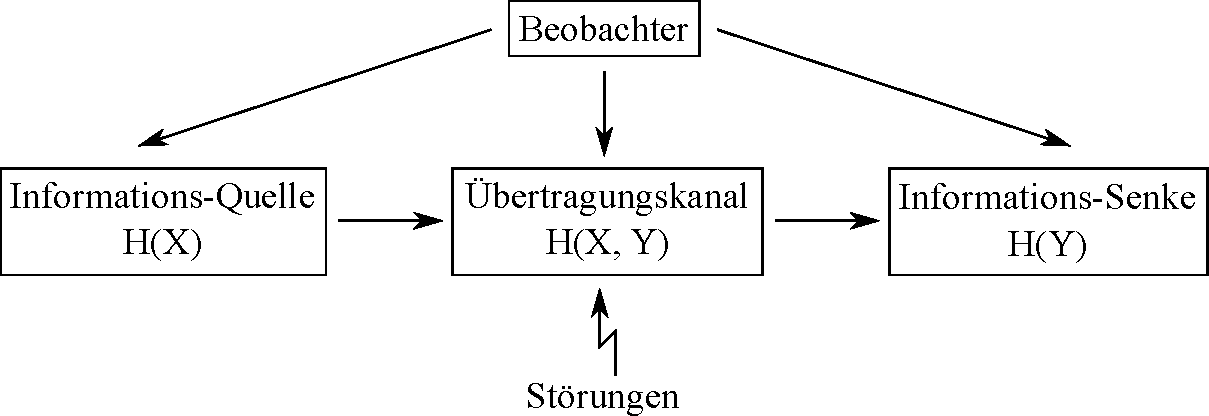
\includegraphics[width=0.8\textwidth]{informationsuebertragung.pdf}
	\caption{Betrachtung der Informationsübertragung als neutraler Beobachter}
	\label{iübertragung}
\end{figure}

Bei einer störungsfreien Übertragung gilt müssen die Entropien aller im Modell als Quellen betrachteten Informationsträger gleich sein. 
$$H(X,Y) = H(X) = H(Y)$$
Abbildung \ref{hxEQhy} zeigt die Beziehung der Entropien im Diagramm.

\begin{figure}[htbp] % positioning htbp: h = here; t = top; b bottom; p own page
	\centering
	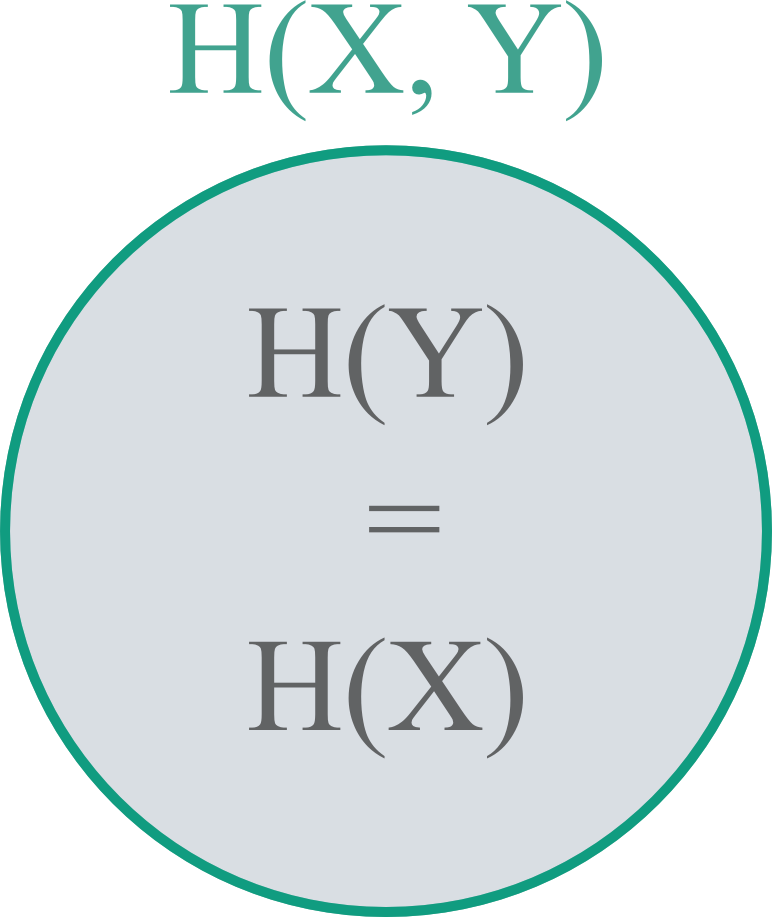
\includegraphics[scale=0.4]{HXgleichHY.png}
	\caption{$H(X)$ gleich $H(Y)$ und damit auch gleich $H(X,Y)$}
	\label{hxEQhy}
\end{figure}

Bei einer vollständig gestörten Übertragung erhält die Informations-Senke völlig andere Informationen als ursprünglich gesendet wurden. Der Beobachter sieht zwei unabhängige Informationsquelen. In diesem Fall ist die Entropie des Übertragungskanals als Verbundquelle maximal und es gilt
$$H(X,Y) = H(X) + H(Y)$$
Abbildung \ref{hxymax} zeigt die Beziehung der Entropien im Diagramm.

\begin{figure}[htbp] % positioning htbp: h = here; t = top; b bottom; p own page
	\centering
	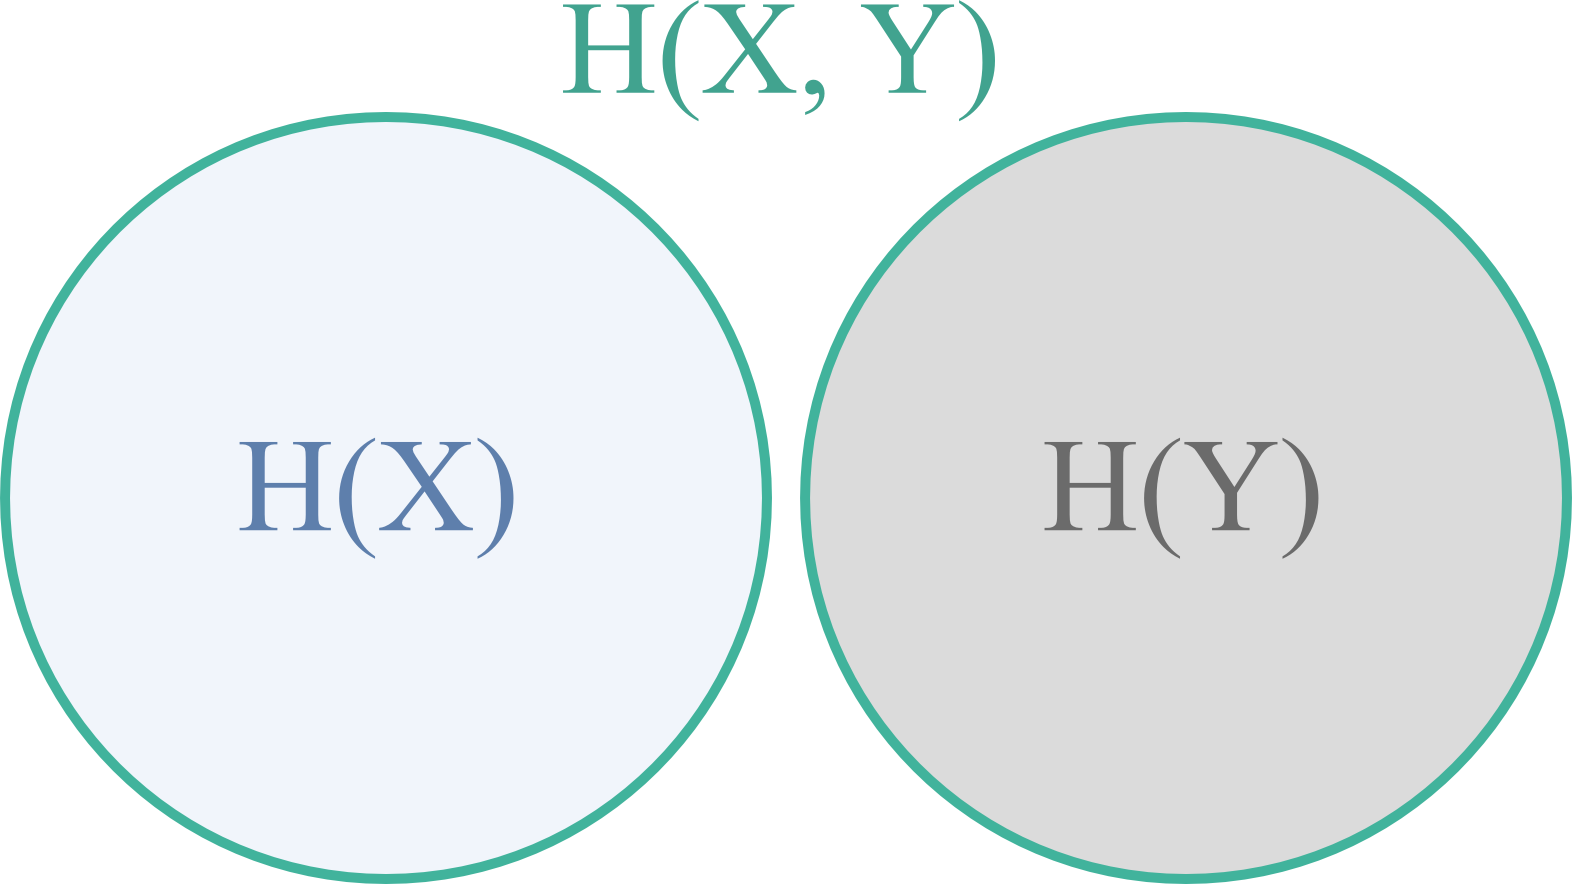
\includegraphics[scale=0.4]{HXYmax.png}
	\caption{$H(X,Y)$ ist maximal}
	\label{hxymax}
\end{figure}

Allgemein schwankt die Entropie der Verbundquelle zwischen maximalem und minimalem Wert je nachdem wie stark die Störungen ausfallen.
$$ H(X) \le H(X,Y) \le H(X) + H(Y) $$
Abbildung \ref{hxymid} zeigt die Beziehung der Entropien im Diagramm.
\begin{figure}[htbp] % positioning htbp: h = here; t = top; b bottom; p own page
	\centering
	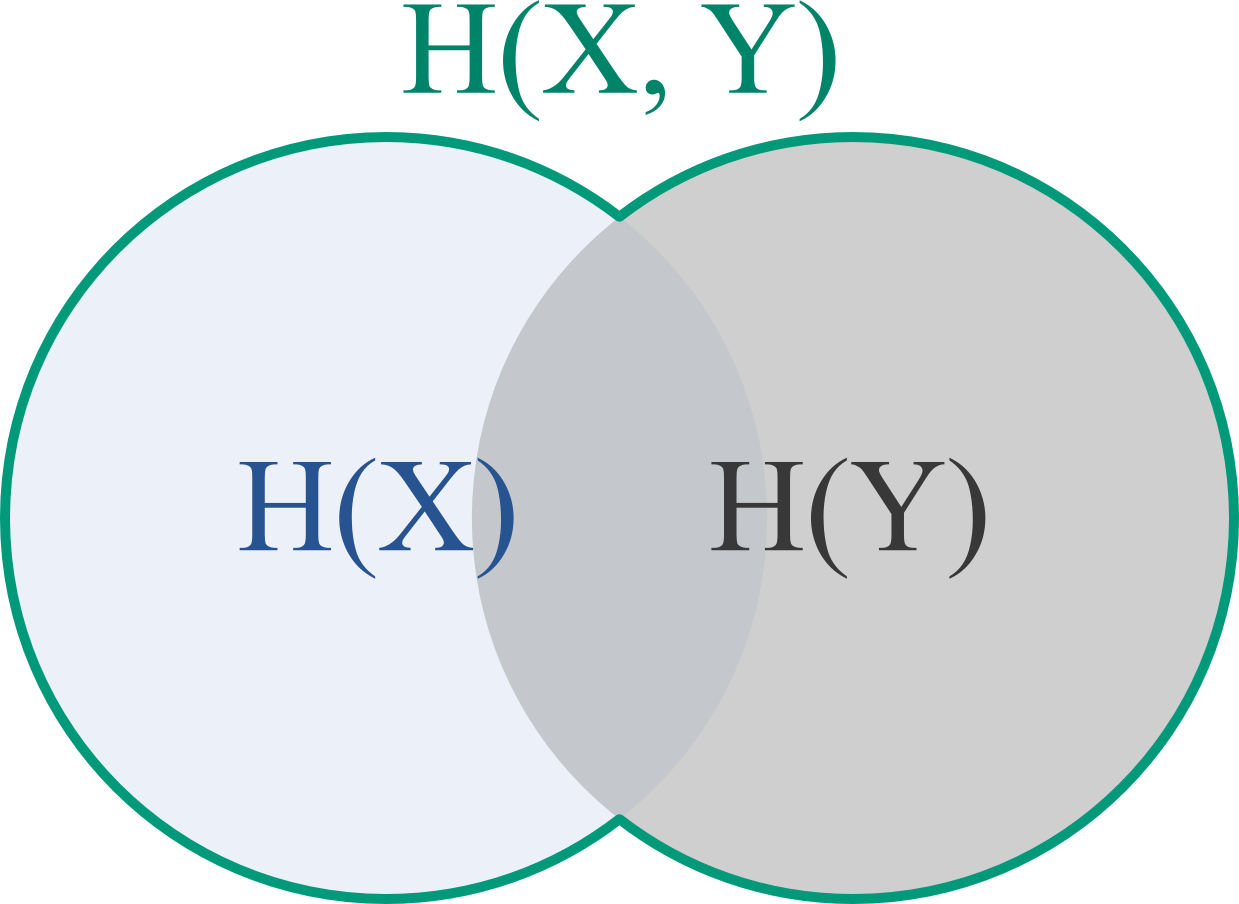
\includegraphics[scale=0.4]{HXYmiddle.png}
	\caption{$H(X,Y)$ zwischen maximalem und minimalem Wert}
	\label{hxymid}
\end{figure}

Die bei der Übertragung verloren gegangene Quellinformation wird \textsl{Äquivokation} genannt. Deren Entropie wird mit $H(X \backslash Y)$ bezeichnet.\footnote{$H(X \backslash Y)$ lies "`Entropie von X ohne Y"'} Die Entropie der Äquivokation lässt sich berechnen mit:
$$ H(X \backslash Y) = H(X, Y) - H(Y) $$

Information, die bei der Übertragung durch Störungen hinzu gefügt wurde, wird \textit{Irrelevanz} genannt. Die Bezeichnung der Entropie der Irrelevanz ist $H(Y \backslash X)$ und wird wie folgt berechnet:
$$H(Y \backslash X) = H(X, Y) - H(X)$$

Die \textsl{Transinformation} ist die Information, welche von der Quelle an den Empfänger tatsächlich übertragen wurde. Die Tansinformation ist die Schnittmenge der Quellinformation mit der empfangenen Information. Die Entropie der Transinformation wird mit $H(X;Y)$ bezeichnet und wie folgt berechnet: 
\begin{align*}
	H(X;Y) &= H(X,Y) - H(X \backslash Y) 
		- H(Y \backslash X) \\
	       &= H(X) + H(Y) - H(X,Y)
\end{align*}

%TODO Kanalkapazität ergänzen

Die Abbildungen \ref{infokanal} und \ref{teilinfo} veranschaulichen die Begriffe Äquivokation, Transinformation und Irrelevanz.
\begin{figure}[htbp] % positioning htbp: h = here; t = top; b bottom; p own page
	\centering
	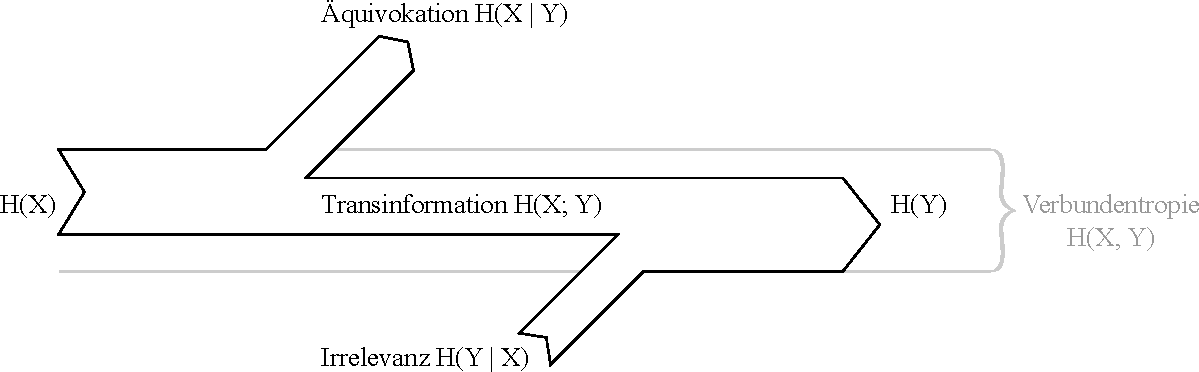
\includegraphics[width = 0.9\textwidth]{informationskanal.pdf}
	\caption{Betrachtung des Informationskanals mit entsprechenden Teilinformationen Äquivokation, Transinformation und Irrelevanz}
	\label{infokanal}
\end{figure}
\begin{figure}[htbp] % positioning htbp: h = here; t = top; b bottom; p own page
	\centering
	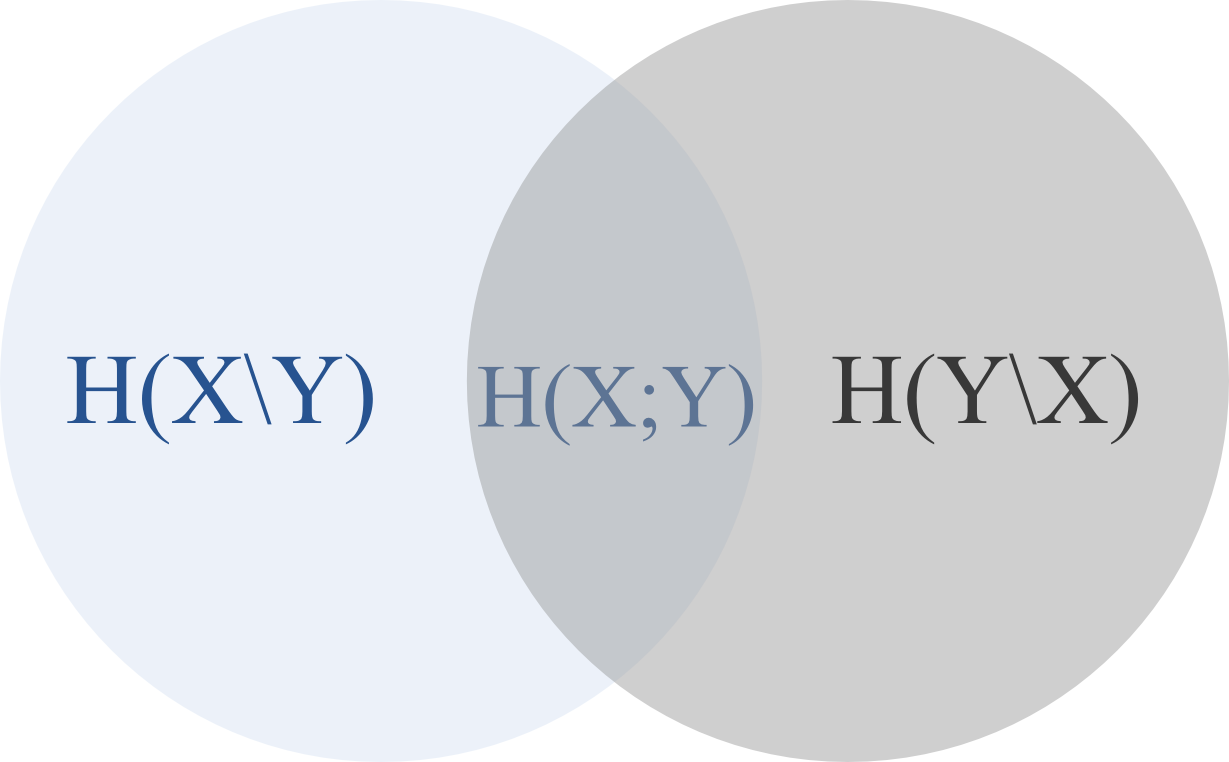
\includegraphics[scale=0.4]{teilinformation.png}
	\caption{Beziehungen der Entropien der Teilinformationen}
	\label{teilinfo}
\end{figure}

%TODO Informationsübertragung Sonderfälle ergänzen

\newpage
\section{Gestörte Übertragungskanäle}
In diesem Abschnitt wird am Beispiel eines symmetrisch gestörten Übertragungskanals die Analyse der Entropien durchgeführt. Es wird eine Quelle $X$ mit dem Binäralphabet $A = \{a_1,a_2\}$ betrachtet. Die Quelle $X$ und die Senke $Y$ mit dem Alphabet $B = \{b_1, b_2\}$ sind über folgende Wahrscheinlichkeitsfelder allgemein definiert:
$$
	X =
	\left(
	\begin{array}{cc}
		a_1    & a_2 \\
		P(a_1) & 1-P(a_1)
	\end{array}
	\right)
	\hspace{1cm}
	Y = 
	\left(
	\begin{array}{cc}
		b_1    & b_2 \\
		P(b_1) & 1-P(b_1)
	\end{array}
	\right)
$$

Bei Fehlerfreier Übertragung entspricht das Zeichen $a_1$ dem Zeichen $b_1$ und $a_2$ entspricht $b_2$. Die Wahrscheinlichkeit, dass ein Zeichen einem falschen Zeichen zugeordnet wird, weil es sich hier um Binäralphabete handelt, Bitfehlerwahrscheinlichkeit $P_f$ genannt. Dass statt $a_1$ $b_2$ beim Empfänger empfangen wird geschieht mit Wahrscheinlichkeit $P(a_1 \mid b_2)$. Die Bezeichnung $P(a_1 \mid b_2)$ beschreibt das Ereignis, dass bei der Übertragung $a_1$ gesendet und $b_2$ empfangen wird. Entsprechend gilt für $P(a_1 \mid b_1)$ die Wahrscheinlichkeit, dass wenn $a_1$ gesendet wird auch $b_1$ empfangen wird. Da die Bitfehlerwahrscheinlichkeit in diesem Beispiel symmetrisch ist gilt:
$$ P(a_1 \mid b_2) = P(a_2 \mid b_1) = P_f $$

Das die unterschiedlichen Ereignisse im Diagramm dargestellt zeigt Abbildung \ref{symStoerung}. Die Pfeile zeigen mit ihrer Beschriftung, wie die Wahrscheinlichkeiten bezeichnet werden und wie diese in diesem Beispiel zusammenhängen. 
\begin{figure}[htbp] % positioning htbp: h = here; t = top; b bottom; p own page
	\centering
	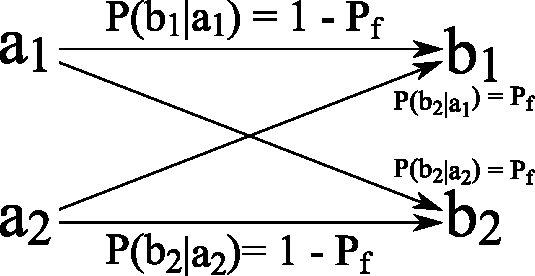
\includegraphics[scale=.8]{symmetrischeStoerung.pdf}
	\caption{Wahrscheinlichkeiten bei der Übertragung der Zeichen}
	\label{symStoerung}
\end{figure}
Im folgenden wird das Wahrscheinlichkeitsfeld der Verbundquelle erstellt, also der Quelle in der wir Infermationserzeuger und -Empfänger gemeinsam betrachten. Jede Wahrscheinlichkeit eines Ereignisses berechnet sich aus der Wahrscheinlichkeit, dass die Quelle ein bestimmtes Zeichen sendet und der Wahrscheinlichkeit, dass dieses Zeichen als solches empfangen oder verfälscht wird. Für das Zeichen $a_1$ werden so die Wahrscheinlichkeiten der beiden Ereignisse berechnet, dass entweder das Zeichen $b_1$ oder das Zeichen $b_2$ empfangen wird. Es gibt also folgende vier Ereignisse:
\begin{center}
	\begin{tabular}{cc}
		$a_1$ wird gesendet und $b_1$ empfangen & $P(a_1) \cdot P(b_1 \mid P(a_1))$ \\
		$a_1$ wird gesendet und $b_2$ empfangen & $P(a_1) \cdot P(b_2 \mid P(a_1))$ \\
		$a_2$ wird gesendet und $b_2$ empfangen & $P(a_2) \cdot P(b_2 \mid P(a_2))$ \\
		$a_2$ wird gesendet und $b_1$ empfangen & $P(a_2) \cdot P(b_1 \mid P(a_2))$ \\ 
	\end{tabular}
\end{center}

Als Beobachter gilt für den Kanal $K$ also das Wahrscheinlichkeitsfeld:
$$
	K = 
	\left(
	\begin{array}{*{4}{c}}
		a_1b_1                          & a_2b_2           & a_1b_2                    & a_2b_1 \\
		P(a_1) P(b_1 \mid P(a_1)) & P(a_2) P(b_2 \mid a_2) & P(a_1) P(b_2 \mid P(a_1)) & P(a_2) P(b_1 \mid P(a_2)) \\
	\end{array}
	\right)
$$

%TODO Rauschmatrix Ü?

Das Wahrscheinlichkeitsfeld kann auch als Verbundmatrix $V$ geschrieben werden:
\begin{align*}
	V &= \left(
	     \begin{array}{*{2}{c}}
	     	P(a_1,b_1) & P(a_1,b_2) \\
	     	P(a_2,b_1) & P(a_2,b_2) \\
	     \end{array}
	     \right) \\
	  &= \left(
	     \begin{array}{*{2}{c}}
	     	P(a_1) P(b_1 \mid P(a_1)) & P(a_1) P(b_2 \mid P(a_1)) \\
	     	P(a_2) P(b_1 \mid P(a_2)) & P(a_2) P(b_2 \mid P(a_2)) \\
	     \end{array}
	     \right) \\
\end{align*}

Aus der Vernundmatrix lassen sich die Wahrscheinlichkeiten der Quellenzeichen über die Summe der Zeilen rückberechnen. Dies gilt, da die Ereignisse je Spalte alle dem Ereignis, dass ein bestimmtest Zeichen gesendet wurde, zuzuordnen sind. Ebenso gilt, dass die Wahrscheinlichkeiten für die empfangenen Zeichen sich über die Summe der jeweiligen Spalten ergeben.

Die Entropie einer Quelle ist maximal, wenn jedes Zeichen des Alphabetes gleich wahrscheinlich generiert werden. Für die Quelle wird die maximale Entropie $H(X) = 1$ angenommen. Also muss $P(a_1) = \frac{1}{2}$ und $P(a_2) = \frac{1}{2}$ gelten. Da die Störungen symmetrisch wirken muss auch $P(b_1) = \frac{1}{2}$ und $P(b_2) = \frac{1}{2}$ gelten. Damit ergibt sich für die Verbundmatrix:

$$
V = 
\left(
\begin{array}{*{2}{c}}
 	\frac{1-P_f}{2} & \frac{P_f}{2} \\
 	\\
 	\frac{P_f}{2}   & \frac{1-P_f}{2} \\
\end{array}
\right)
$$

Die Verbundentropie $H(X,Y)$ ist in diesem Beispiel also:
\begin{align*}
	H(X,Y) &= \sum_{i=1}^2\sum_{j=1}^2
		P(a_i,b_j) \cdot ld \left( 
		\frac{1}{P(a_i,b_j)} \right) \\
		   &= 2 \cdot \frac{1-P_f}{2} 
		\cdot ld \left( 
		\frac{2}{1-P_f} \right) 
		+ 2 \cdot \frac{P_f}{2} 
		\cdot ld \left( 
		\frac{2}{P_f} \right)\\
		   &= (1-P_f) \cdot ld \left( 
		\frac{2}{1-P_f} \right) 
		+ P_f	\cdot ld \left( 
		\frac{2}{P_f} \right)\\
		   &= (1-P_f) \cdot (ld(2) - ld(1-P_f)) 
		+ P_f	\cdot (ld(2) - ld(P_f))\\
		   &= (1-P_f) \cdot (1 - ld(1-P_f)) 
		+ P_f	\cdot (1 - ld(P_f))\\
		   &= (1 - P_f) - (1 - P_f)ld(1-P_f) 
		+ P_f - P_fld(P_f)\\
		   &= 1 - (1 - P_f)ld(1-P_f) - P_fld(P_f)\\
\end{align*}

Die Transinformation ergibt sich aus:
\begin{align*}
	H(X;Y) &= H(X) + H(Y) - H(X,Y) \\
	       &= 1 + 1 - (1 - (1 - P_f)
	       ld(1-P_f) - P_fld(P_f))\\
	       &= 1 + 1 - 1 + (1 - P_f)
	       ld(1-P_f) + P_fld(P_f))\\
	       &= 1 + (1 - P_f)
	       ld(1-P_f) + P_fld(P_f))\\
\end{align*}

Für die Äquivokation folgt:
\begin{align*}
	H(X \backslash Y) &= H(X, Y) - H(Y) \\
	&= 1 - (1 - P_f)ld(1-P_f) 
	- P_fld(P_f) - 1\\
	&= -(1 - P_f)ld(1-P_f) - P_fld(P_f) \\
\end{align*}

Für die Irrelevanz gilt:
\begin{align*}
	H(Y \backslash X) &= H(X, Y) - H(X) \\
	&= 1 - (1 - P_f)ld(1-P_f) 
	- P_fld(P_f) - 1\\
	&= -(1 - P_f)ld(1-P_f) - P_fld(P_f) \\
\end{align*}

Praktischer Weise ist die Transinformation für $P_f = 1$ und $P_f = 0$ maximal. Dies ist sinnvoll, da bei völliger Störung ($P_f = 1$) jedes Bit invertiert wird. Um die ursprüngliche Information zu erhalten reicht es das Bitmuster zu invertieren.

%TODO Optimalcodes / Quellencodierung Einführung ergänzen
%TODO Aufbau von Optimalcodes und Kraft Ungleichung ergänzen
%TODO Shannon-Code ergänzen (nicht klausurrelevant)

\section{Konstruktion von binären Optimalcodes}
\subsection{Fano-Code}
Konstruktionsmethode:
\begin{enumerate}
\item Sortiere abfallend die zu codierenden Zeichen nach deren Wahrscheinlichkeiten.
\item Teile die Gruppe der Zeichen in zwei Gruppen, wobei die Summe der Wahrscheinlichkeiten der einen Gruppe möglichst der Summe der Wahrscheinlichkeiten der anderen Gruppe entspricht. Einer Gruppe wird die $0$ der anderen die $1$ als erste Stelle im Codewort zugeordnet.
\item Wiederhole Schritt 2 mit den entstandenen Teilgruppen, wenn die jeweilige Teilgruppe mehr als ein Zeichen enthält. Andernfalls ist dem einzigen Zeichen der Gruppe das entstandene Codewort zuzuordnen.
\end{enumerate}

Beispiel: 
$$
X = 
\left(
\begin{array}{*{7}{c}}
	a_1         & a_2         & a_3         & a_4         & a_5         & a_6          & a_7          \\
	\frac{1}{4} & \frac{1}{4} & \frac{1}{8} & \frac{1}{8} & \frac{1}{8} & \frac{1}{16} & \frac{1}{16} \\
\end{array}
\right)
$$
\begin{itemize}
  \item Die ersten beiden Gruppen sind $\{a_1, a_2\}$ und $\{a_3, \ldots, a_7\}$, da 
	$$ \sum_{i \in \{a_1, a_2\}}P(a_i) = \frac{1}{2} = \sum_{i \in \{a_3, \ldots, a_7\}} P(a_i) $$
  \item $\{a_1, a_2\}$ wird als erste Ziffer 0 und $\{a_3, \ldots, a_7\}$ als erste Ziffer 1 zugeordnet.
  \item $\{a_1, a_2\}$ wird aufgeteilt in $a_1$ und $a_2$. 
  \item $a_1$ erhält 0 und $a_2$ 1 als zweite Ziffer. Damit gilt:
	$$ a_1 \mapsto 00 $$
	$$ a_2 \mapsto 01 $$
  \item $\{a_3, \ldots, a_7\}$ wird aufgeteilt in $\{a_3, a_4\}$ und $\{a_5, a_6, a_7\}$, da
  $$ \sum_{i \in \{a_3, a_4\}}P(a_i) = \frac{1}{4} = \sum_{i \in \{a_5, a_6, a_7\}} P(a_i) $$
  \item $\{a_3, a_4\}$ wird 0 und $\{a_5, a_6, a_7\}$ als zweite Ziffer 1 zugeordnet.
  \item $\{a_3, a_4\}$ wird aufgeteilt in $a_3$ und $a_4$.
  \item $a_3$ erhält 0 und $a_2$ 1 als dritte Ziffer. Damit gilt:
	$$ a_3 \mapsto 100 $$
	$$ a_4 \mapsto 101 $$
  \item $\{a_5, a_6, a_7\}$ wird aufgeteilt in $a_5$ und $\{a_6, a_7\}$, da
  $$ P(a_5) = \frac{1}{8} = P(a_6) + P(a_7) $$
  \item $a_5$ erhält 0 und $\{a_6, a_7\}$ 1 als dritte Ziffer. Damit gilt:
	$$ a_5 \mapsto 110 $$
  \item $\{a_6, a_7\}$ wird aufgeteilt in $a_6$ und $a_7$.
  \item $a_6$ erhält 0 und $a_7$ 1 als vierte Ziffer. Damit gilt:
	$$ a_6 \mapsto 1110 $$
	$$ a_7 \mapsto 1111 $$
\end{itemize}

Dieselbe Konstruktionsmethode aufgeschrieben in einer Tabelle:

\begin{center}
\begin{tabular}{cc*{4}{c}r}
	$a_i$ & $P(a_i)$       & 1. Aufteilung & 2. Aufteilung & 3. Aufteilung & 4. Aufteilung & Code \\
	      &                & 1.Stelle      & 2. Stelle     & 3. Stelle     & 4. Stelle     &      \\
	$a_1$ & $\frac{1}{4}$  & 0             & 0             &               &               & 00   \\
	$a_2$ & $\frac{1}{4}$  & 0             & 1             &               &               & 01   \\
	$a_3$ & $\frac{1}{8}$  & 1             & 0             & 0             &               & 100  \\
	$a_4$ & $\frac{1}{8}$  & 1             & 0             & 1             &               & 111  \\
	$a_5$ & $\frac{1}{8}$  & 1             & 1             & 0             &               & 110  \\
	$a_6$ & $\frac{1}{16}$ & 1             & 1             & 1             & 0             & 1110 \\
	$a_7$ & $\frac{1}{16}$ & 1             & 1             & 1             & 1             & 1111 \\
\end{tabular}
\end{center}

\subsection{Huffman-Code}
Konstruktionsmethode:
\begin{enumerate}
  \item Sortiere abfallend die zu codierenden Zeichen nach deren Wahrscheinlichkeiten.
  \item Das Zeichen mit der niedrigsten Wahrscheinlichkeit erhält als erste Stelle eine 1. Das Zeichen mit der zweitniedrigsten Wahrscheinlichkeit erhält als erste Stelle eine 0. Die Stellen werden bei diesem Verfahren von rechts nach links angehängt.
  \item Fasse das Zeichen mit der niedrigsten Wahrscheinlichkeit und das Zeichen mit der zweitniedrigsten Wahrscheinlichkeit in einer Gruppe zusammen.
  \item Ordne der Gruppe die Summe der Wahrscheinlichkeiten der Zeichen, die der Gruppe angehören zu.
  \item Gruppen mit ihren zugeordneten Wahrscheinlichkeiten sind wie Zeichen zu behandeln. Gruppen können ebenso, wie Zeichen, zu größeren Gruppen zusammengefasst werden. Zusammengefassten Gruppen wird ebenso die Summe der Wahrscheinlichkeiten der kleineren Gruppen, aus denen sie bestehen, zugeordnet. Wiederhole alle Schritte bis eine einzige große Gruppe übrig ist.
\end{enumerate}

Beispiel: 
$$
X = 
\left(
\begin{array}{*{7}{c}}
	a_1         & a_2         & a_3         & a_4         & a_5         & a_6          & a_7          \\
	\frac{1}{4} & \frac{1}{4} & \frac{1}{8} & \frac{1}{8} & \frac{1}{8} & \frac{1}{16} & \frac{1}{16} \\
\end{array}
\right)
$$
\begin{itemize}
  \item Absteigende Sortierung nach Wahrscheinlichkeiten ist
  $$((a_1,1/4), (a_2,1/4), (a_3,1/8), (a_4,1/8), (a_5,1/8), (a_6,1/16), (a_7,1/16))$$
  \item $a_6$ wird als erste Stelle 0 und $a_7$ wird als erste Stelle 1 zugeordnet.
  $$ a_6 \mapsto 0 $$
  $$ a_7 \mapsto 1 $$
  \item $a_6$ und $a_7$ werden in einer Gruppe zusammengefasst. Der Gruppe wird die Wahrscheinlichkeit $1/16 + 1/16 = 1/8$ zugeordnet.

  \item Absteigende Sortierung nach Wahrscheinlichkeiten ist
  $$((a_1,1/4), (a_2,1/4), (\{a_6, a_7\},1/8) (a_3,1/8), (a_4,1/8), (a_5,1/8))$$
  \item $a_4$ erhält als erste Stelle 0 und $a_5$ erhält als erste Stelle 1.
  $$ a_4 \mapsto 0 $$
  $$ a_5 \mapsto 1 $$
  \item $a_4$ und $a_5$ werden in einer Gruppe zusammengefasst. Der Gruppe wird die Wahrscheinlichkeit $1/8 + 1/8 = 1/4$ zugeordnet.

  \item Absteigende Sortierung nach Wahrscheinlichkeiten ist
  $$((\{a_4,a_5\},1/4),(a_1,1/4), (a_2,1/4), (\{a_6, a_7\},1/8) (a_3,1/8))$$
  \item $\{a_6, a_7\}$ erhalten jeweils als zweite Stelle 0 und $a_3$ erhält als erste Stelle 1.
  $$ a_6 \mapsto 00 $$
  $$ a_7 \mapsto 01 $$
  $$ a_3 \mapsto 1 $$
  \item $\{a_6, a_7\}$ und $a_3$ werden in einer Gruppe zusammengefasst. Der Gruppe wird die Wahrscheinlichkeit $1/8 + 1/8 = 1/4$ zugeordnet.
  
  \item Absteigende Sortierung nach Wahrscheinlichkeiten ist
  $$((\{a_6, a_7, a_3\},1/4),(\{a_4,a_5\},1/4),(a_1,1/4), (a_2,1/4))$$
  \item $a_1$ erhält als erste Stelle 0 und $a_2$ erhält als erste Stelle 1.
  $$ a_1 \mapsto 0 $$
  $$ a_2 \mapsto 1 $$
  \item $a_1$ und $a_2$ werden in einer Gruppe zusammengefasst. Der Gruppe wird die Wahrscheinlichkeit $1/4 + 1/4 = 1/2$ zugeordnet.
  
  \item Absteigende Sortierung nach Wahrscheinlichkeiten ist
  $$((\{a_1, a_2\},1/2),(\{a_6, a_7, a_3\},1/4),(\{a_4,a_5\},1/4))$$
  \item $\{a_6, a_7, a_3\}$ erhalten als weitere Stelle 0 und $\{a_4,a_5\}$ erhalten als weitere Stelle 1.
  $$ a_6 \mapsto 000 $$
  $$ a_7 \mapsto 001 $$
  $$ a_3 \mapsto 01 $$
  $$ a_4 \mapsto 10 $$
  $$ a_5 \mapsto 11 $$
  \item $\{a_6, a_7, a_3\}$ und $\{a_4,a_5\}$ werden in einer Gruppe zusammengefasst. Der Gruppe wird die Wahrscheinlichkeit $1/4 + 1/4 = 1/2$ zugeordnet.
  
  \item Absteigende Sortierung nach Wahrscheinlichkeiten ist
  $$((\{a_6, a_7, a_3, a_4, a_5\},1/2),(\{a_1, a_2\},1/2))$$
  \item $\{a_6, a_7, a_3, a_4, a_5\}$ erhalten als weitere Stelle 0 und $\{a_1, a_2\}$ erhalten als weitere Stelle 1.
  $$ a_6 \mapsto 0000 $$
  $$ a_7 \mapsto 0001 $$
  $$ a_3 \mapsto 001 $$
  $$ a_4 \mapsto 010 $$
  $$ a_5 \mapsto 011 $$
  $$ a_1 \mapsto 10 $$
  $$ a_2 \mapsto 11 $$
  \item $\{a_6, a_7, a_3, a_4, a_5\}$ und $\{a_1, a_2\}$ werden in einer Gruppe zusammengefasst. Der Gruppe wird die Wahrscheinlichkeit $1/2 + 1/2 = 1$ zugeordnet. Die Konstruktion ist abgeschlossen, da eine einzige Gruppe übrig ist.
\end{itemize}

Da bei diesem Verfahren kein Codewort erzeugt wird, das im Präfix eines anderen Codewortes enthalten ist, kann beim einlesen einer Zeichenkette eindeutig direkt entschieden werden um welches Zeichen es sich jeweils handelt.
%\begin{center}
%\begin{tabular}[t]{lccc}
%$a_i \mapsto code$ & Gruppe & $P$  & Zuordnung \\
%$a_1 \mapsto $     & $a_1$  & 1/4  &           \\
%$a_2 \mapsto $     & $a_2$  & 1/4  &           \\
%$a_3 \mapsto $     & $a_3$  & 1/8  &           \\
%$a_4 \mapsto $     & $a_4$  & 1/8  &           \\
%$a_5 \mapsto $     & $a_5$  & 1/8  &           \\
%$a_6 \mapsto $     & $a_6$  & 1/16 & 0         \\
%$a_7 \mapsto $     & $a_7$  & 1/16 & 1         \\
%\end{tabular}
%
%\begin{tabular}[t]{lccc}
%$a_i \mapsto code$ & Gruppe & $P$  & Zuordnung \\
%$a_1 \mapsto $     & $a_1$  & 1/4  &           \\
%$a_2 \mapsto $     & $a_2$  & 1/4  &           \\
%                   & $\{a_6,a_7\}$ &           \\
%$a_3 \mapsto $     & $a_3$  & 1/8  &           \\
%$a_4 \mapsto $     & $a_4$  & 1/8  &         0 \\
%$a_5 \mapsto $     & $a_5$  & 1/8  &         1 \\
%$a_6 \mapsto 0$                                \\
%$a_7 \mapsto 1$                                \\
%\end{tabular}
%
%\begin{tabular}[t]{lccc}
%$a_i \mapsto code$ & Gruppe & $P$  & Zuordnung \\
%$a_1 \mapsto $     & $a_1$  & 1/4  &           \\
%$a_2 \mapsto $     & $a_2$  & 1/4  &           \\
%                   & $\{a_6,a_7\}$ &           \\
%$a_3 \mapsto $     & $a_3$  & 1/8  &           \\
%$a_4 \mapsto 0$                                \\
%$a_5 \mapsto 1$                                \\
%$a_6 \mapsto 0$                                \\
%$a_7 \mapsto 1$                                \\
%\end{tabular}
%\end{center}

